\subsection{Stochastic Model - Step Response}
In this exercise it is desired to simulate the non-linear model with the stochastic variables. For doing this, the chosen noise contributions can be seen below. It should be notice that the state noise is relative to the mass in gram, and is only a contribution to the unknown disturbance, as seen in \cref{eq:stoc_states} in \cref{sec:Stoc_Model}, and therefore it is only a 2x2 matrix. The measurement noise is relative to the height, which is in cm. All the noise contributions is assumed to be uncorrelated.
\begin{equation}
    \begin{matrix}
        R_{x,low} =\begin{bmatrix}
             5 & 0\\
             0 & 10
        \end{bmatrix} &
        R_{x,medium} =\begin{bmatrix}
            50 & 0\\
            0 & 100
        \end{bmatrix} &
        R_{x,high} =\begin{bmatrix}
            500 & 0\\
            0 & 1000
        \end{bmatrix} \\
        R_{y,low} =\begin{bmatrix}
             0.2 & 0 \\
             0 & 0.4 \\
        \end{bmatrix} &
        R_{y,medium} =\begin{bmatrix}
             1 & 0 \\
             0 & 2 \\
        \end{bmatrix} &
        R_{y,high} =\begin{bmatrix}
             5 & 0 \\
             0 & 10 \\
        \end{bmatrix} &
    \end{matrix}
    \label{eq:Noise_values}
\end{equation}
The response of the simulation with a step of 10, 25 and 50\% can be seen in \cref{fig:stoc_step_10}, \cref{fig:stoc_step_25} and \cref{fig:stoc_step_50} respectively. In these cases, the system is initialized at steady state.
\begin{figure}[H]
    \centering
    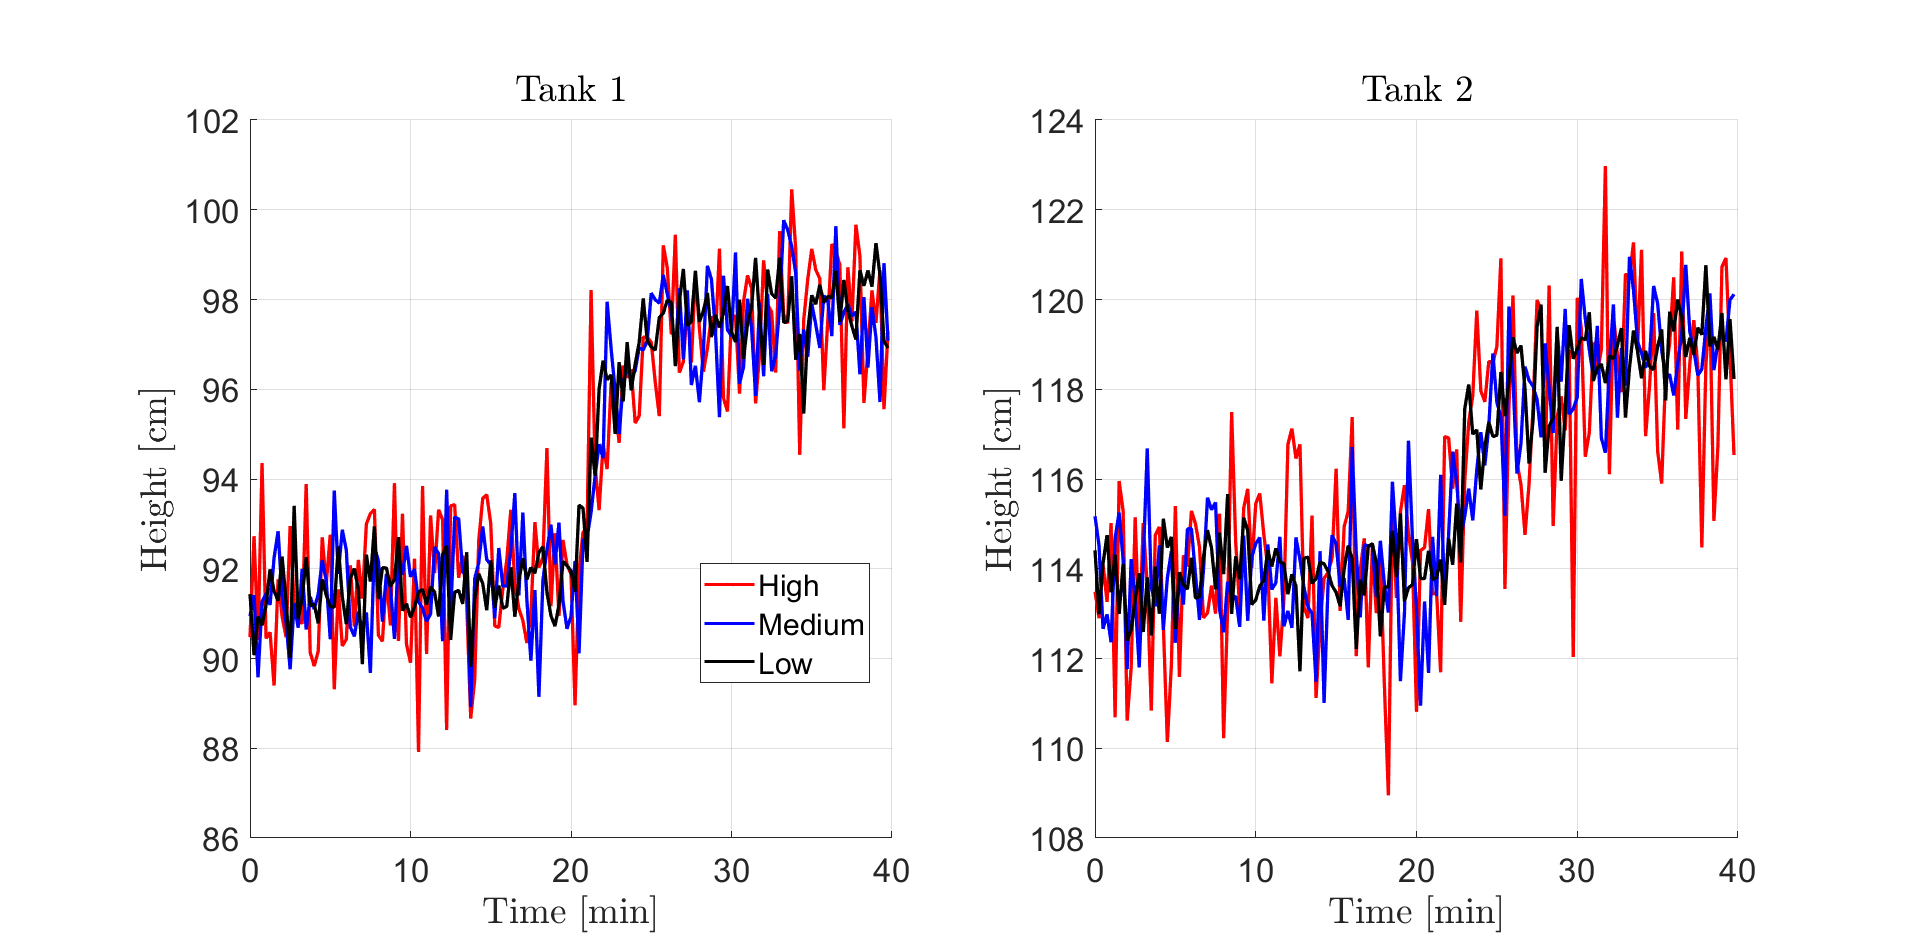
\includegraphics[width=1\textwidth]{Figures/Pr3.2_Stoc_step10.png}
    \caption{Step 10 \% on $u_1$ - Stochastic model}
    \label{fig:stoc_step_10}
\end{figure}
\begin{figure}[H]
    \centering
    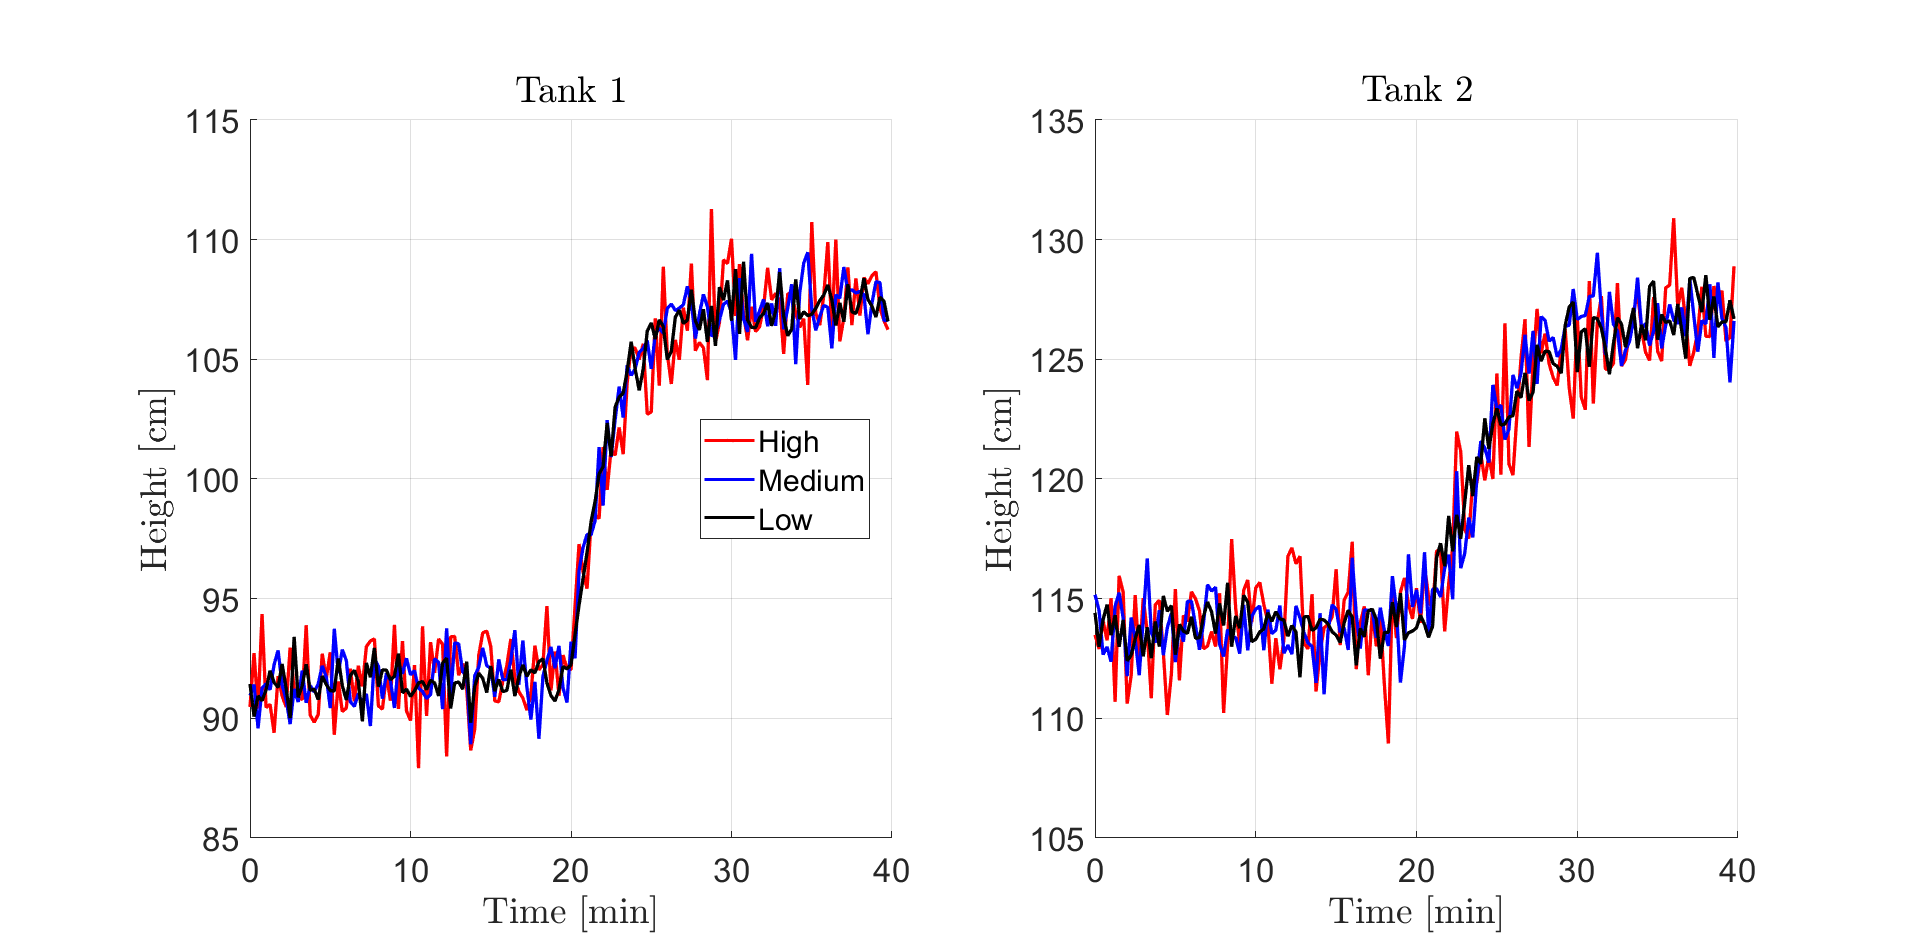
\includegraphics[width=1\textwidth]{Figures/Pr3.2_Stoc_step25.png}
    \caption{Step 25 \% on $u_1$ - Stochastic model}
    \label{fig:stoc_step_25}
\end{figure}
\begin{figure}[H]
    \centering
    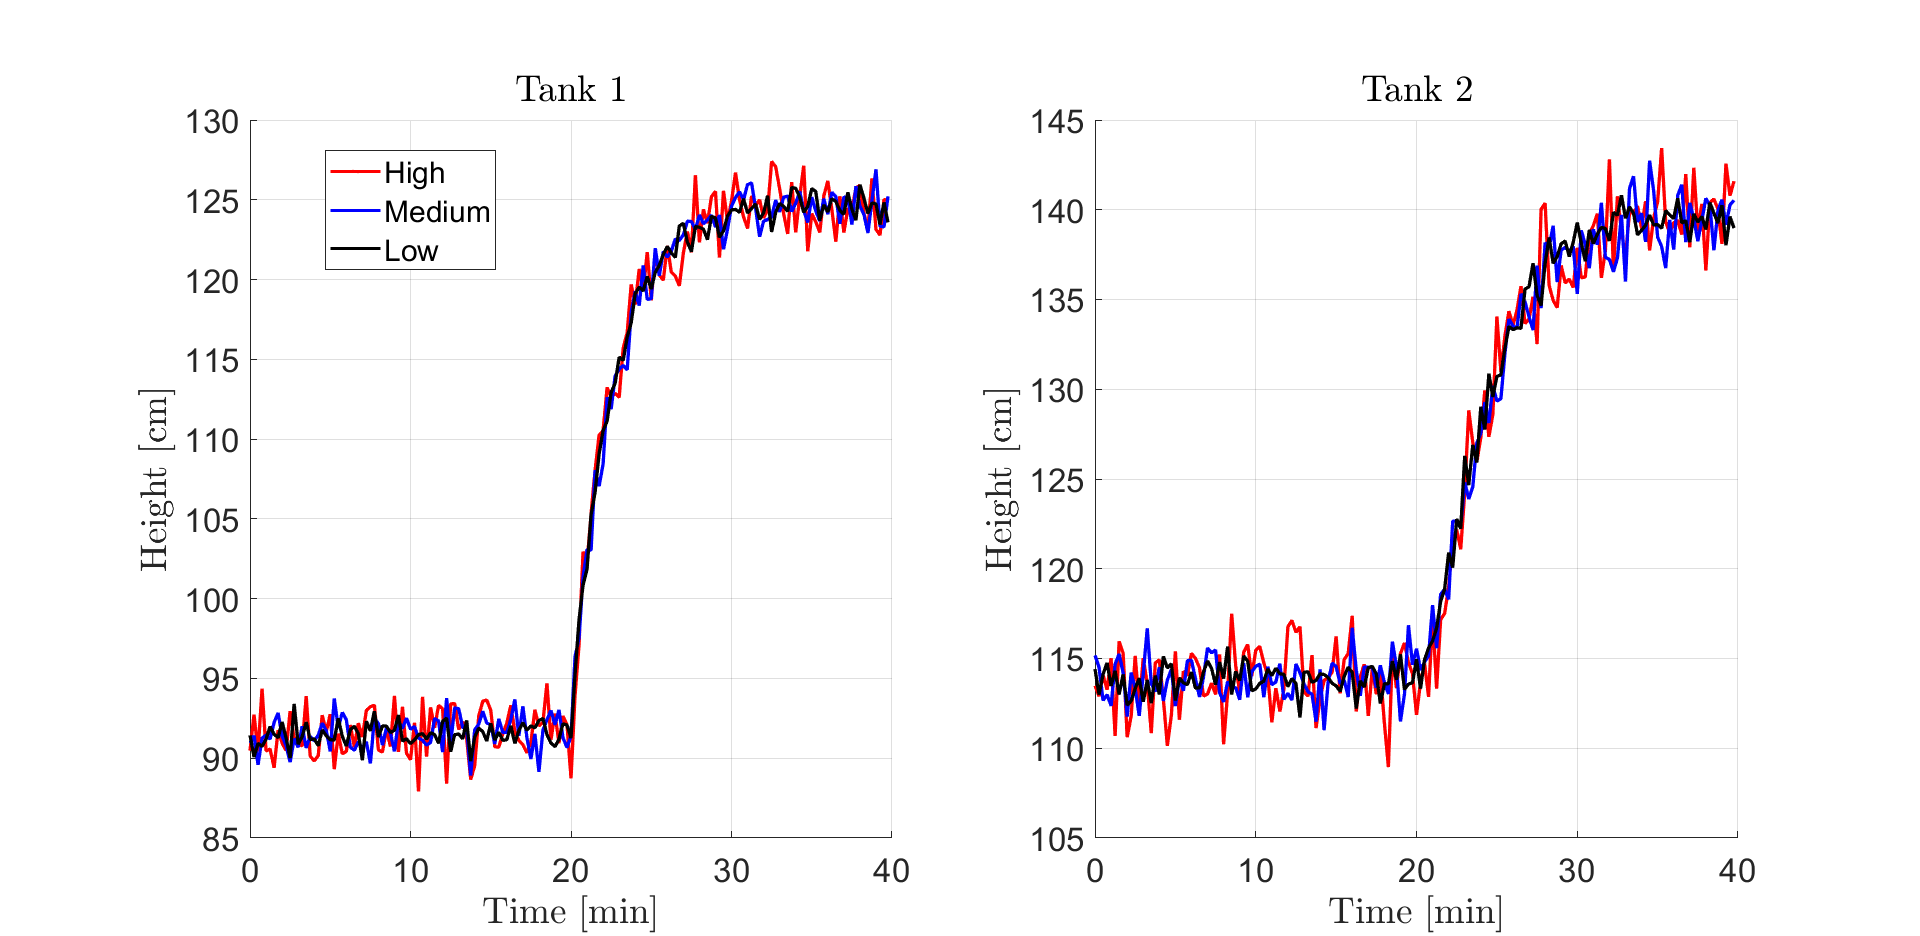
\includegraphics[width=1\textwidth]{Figures/Pr3.2_Stoc_step50.png}
    \caption{Step 50 \% on $u_1$ - Stochastic model}
    \label{fig:stoc_step_50}
\end{figure}
The 3 noise affections is clearly seen for each step, and the larger the step, the noise contribution has a smaller relative effect.